\label{capitolo1}
\section{Progettazione a basso consumo di potenza}
Nel corso degli anni ci si è spostati verso la progettazione di sistemi hardware che consumassero sempre meno. Le motivazioni che hanno portato a questa evoluzione sono molteplici e di diversa natura; alcune di queste sono:
\begin{description}
\item[Tecnologiche:] l'aumento della frequenza e dei transistor presenti nel circuito obbligano ad un minor consumo di energia
\item[Commerciali:] la diffusione di dispositivi portatili che richiedono alte prestazioni e un basso consumo energetico
\item[Economiche:] ridurre il costo del \emph{packaging} del comparto batterie
\end{description}
La diffusione di dispositivi portatili ha portato ad avere un \emph{trade-off} tra le performance ed il consumo energetico.\\
Il design a basso consumo e le metodologie di stima del consumo di potenza devono essere valutate ad un diverso livello di astrazione durante tutto il processo di progettazione; i diversi livelli sono
\begin{itemize}
\item System Level
\item Behavioral Level
\item RT (Register Transfer) Level
\item Gate Level
\item Transistor Level
\end{itemize}
L'evoluzione attuale della tecnologia delle batterie è insufficiente rispetto all'evoluzione odierna dei circuiti, infatti, le capacità delle batterie aumentano all'incirca del 10\%-15\% all'anno mentre il consumo dei circuiti aumenta molto più velocemente, questo comporta un gap notevole tra il fabbisogno di potenza dei circuiti e la disponibilità data dai pacchi batterie.\\
Ad oggi la tecnologia più utilizzata per la realizzazione di circuiti digitali è quella \textbf{CMOS} in quanto la velocità di switching è notevole ed il consumo di corrente è intrinsecamente basso.
Il consumo di potenza nei CMOS è dato da 
$$P=P_{switching}+P_{short-circuit}+P_{leakage}$$
Dove $P_{switching}$ è la potenza necessaria per caricare e scaricare il condensatore durante il cambio di contesto del transistor $P_{short-circuit}$ è la corrente che va da $V_{dd}$ a $GND$ durante la transizione di uscita ed infine $P_{leakage}$ è la componente data dalla corrente di leakage.\\
La parte $P_{switching}$ è la parte predominante della dissipazione di potenza e l'obiettivo dei progettisti è quello di minimizzare questo fattore durante la fase di design del sistema. Per quanto riguarda, invece, $P_{short-circuit}$ e $P_{leakage}$ per minimizzarli occorre agire a livello tecnologico e non risulta essere una cosa semplice.\\
\begin{figure}
\centering
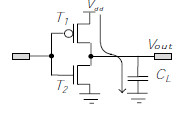
\includegraphics[width=10cm]{img/vddoutput.png}
\label{fig:vddoutput}
\caption{Transizione $0 \rightarrow V_{dd}$}
\end{figure}